\documentclass[11pt,a4paper]{article}
% Modèle de rapport de stage et conseils de rédaction, mise en page...
% L. Bellon, avril 2010

\usepackage{tabularx} % gestion avancée des tableaux
\usepackage{shortcut}
\usepackage{theme}


\begin{document}

% Pour faciliter la mise en forme de la page du titre, on supprime l'indentation automatique en début de paragraphe
\setlength{\parindent}{0pt}

% Pas d'en-tête ni de pied pour la première page
\thispagestyle{empty}


\includegraphics[height=2cm]{figures/ens_ps.png} \hfill 
\includegraphics[height=2cm]{figures/logo_mva.eps}

\vspace{0.5cm}

\begin{tabularx}{\textwidth}{@{} l X l @{} }
{\sc Master MVA / Mathématiques, Vision, Apprentissage} & & Stage 2021--2022 \\
{\it École Normale Supérieure de Paris-Saclay} & & Alexandre \sc Marthe \\
\end{tabularx}

\begin{center}

\vspace{1.5cm}

\rule[11pt]{5cm}{0.5pt}

\textbf{\huge Titre du rapport}

\rule{5cm}{0.5pt}

\vspace{1.5cm}

\parbox{15cm}{\small
\textbf{Résumé} : \it Un résumé de 10 lignes environ du contenu du rapport, permettant de situer le sujet et les résultats principaux du stage. Lorem ipsum dolor sit amet, consectetur adipiscing elit, sed do eiusmod tempor incididunt ut labore et dolore magna aliqua. Ut enim ad minim veniam, quis nostrud exercitation ullamco laboris nisi ut aliquip ex ea commodo consequat. Duis aute irure dolor in reprehenderit in voluptate velit esse cillum dolore eu fugiat nulla pariatur. Excepteur sint occaecat cupidatat non proident, sunt in culpa qui officia deserunt mollit anim id est laborum. Sed ut perspiciatis unde omnis iste natus error sit voluptatem accusantium doloremque laudantium, totam rem aperiam, eaque ipsa quae ab illo inventore veritatis et quasi architecto beatae vitae dicta sunt explicabo.
} %fin de la commande \parbox du résumé


\vspace{0.5cm}

\parbox{15cm}{
\textbf{Mots clefs} : \it 4 à 5 mots clefs
} %fin de la commande \parbox des mots clefs

\vspace{0.5cm}

\parbox{15cm}{
Stage encadré par :

{\bf Aurelien Garivier}

\href{mailto:aurelien.garivier@ens-lyon.fr}{\tt aurelien.garivier@ens-lyon.fr} / tél. (+33) 4 72 72 81 08

UMPA, ENS de Lyon

{\it 46, allée d’Italie

69364 Lyon Cedex 07, FRANCE}

\url{http://www.umpa.ens-lyon.fr}
} %fin de la commande \parbox encadrant / laboratoire d'accueil

\vspace{1.5cm}


\includegraphics[height=3cm]{figures/logo_umpa.jpg}

\end{center}

\vfill
\hfill \today
 
% Pas d'entéte ni de pied pour la page de sommaire
\thispagestyle{empty}
\section*{Acknowledgment}
I would like to first thank Aurelien Garivier for supervising me, guiding me throughout all the internship, but also for invitation to the summer school and the statistical conference. I got the opportunity to meet many people working close to my research area, and to discover tangent research subjects. I would also like to thank the team I was with at the ENS, Antoine, Aymen and Hugues, with who I shared many great moment, be it social or studious. And finally I would also like to thank the UMPA team as a whole, for welcoming me and making me immediatly feel at ease in the lab.

\tableofcontents
\newpage

% Première page du rapport
\setcounter{page}{1}

% on rétablit l'indentation automatique en début de paragraphe 
\setlength{\parindent}{16pt}

\section{Introduction}
%présenter le reinforcement learning, les applications, les limites actuelles

%intro ML
In the last decade, Machine Learning has become a major field of interest in current scientific research, and has allowed for uncountable technological breakthroughs. Its techniques allows for automisation of many task that usually had to be done by hand by a human. We can find its application everywhere in today’s world. Its strengh is to be able to solve complex problems for which we don’t know an exact solution, by learning through examples and/or training. The main challenges of the field is to find what can be learned, and how it can be learned. Depending on the kind of tasks we want to solve, there are different subdomain of Machine Learning. In this report, we will focus on what is called \emph{Reinforcement Learning}.

%intro RL
Reinforcement Learning is the subfield that investigates how to learn and adapt in real time. The principle is the same as how humans learn to do certain tasks: through trials and errors. It’s for instance the paradigm used in recommandation systems or in the programs that beat humans in board games such as Chess or Go.
The main ideas are quite old\cite{bellman1966dynamic}\cite{bertsekas2012dynamic}, but it gained a lot of hype when it started being associated with deep learning methods, which made it scalable to real world applications. Among the breakthroughs that brought a lot of interest in the field, we can find the development of Deepmind’s Alphago, an algorithm that beat the world’s best Go players, one of the last board games on which humans were still better than machines. Reinforcement Learning methods have been increasingly popular in many different domains, such as scheduling, robot control and telecommunications.

%principle of RL
All those algorithms work on the same principle: optimizing a reward. Similarly to what happens in our brain, where our actions are mainly chosen in a way to maximise the dopamine produced, the algorithms chose actions depending on which will give the best reward. In the example of Chess or Go, the algorithm will receive a positive reward when winning the game, and a penalty when loosing. It could also be designed so that it gain/loses reward when taking/losing a piece. The reward is usually defined by hand depending on the objective. It is then for the algorithm to find the best sequence of actions in order to maximize the reward.

%Sensitive RL
However, in many real world applications, the reward can be stochastic (for instance with only partial observation of the context) and thus, performing the same sequence of actions may not always lead to the same reward. This is why most of the research focus the maximisation of the expected reward, which works very well in practice.
Though, some Reinforcement Learning algorithms can also be found in quite sensitive applications, like software driving autonomous vehicles. The issues with those software is that depending on the action chosen and the context, there could be incidents, such as a car crash and or death of person. As this should be avoided as much as possible, it is mandatory to make the safest algorithm possible. Doing so by defining specific rewards is particularly difficult, as it’s most of the time impossible to predict the exact behavior of the algorithm solely with the rewards. This justifies a need of research in minimizing some risks in Reinforcement Learning. This branch is called Risk-sensitive Reinforcement Learning, and is almost as old as the first formalization of Reinforcement Learning.
\\%s’inspirer de morimura

%intro distributionnal and risk-sensitive RL
There are different approaches in Risk-Sensitive RL. The one that we will get interest in have been tried the first time by \cite{morimura_parametric_2012}[Morimura et al.], which will be detailed later.
\\

In this report we will start by recalling the main results in Reinforcement Learning for known environement, later we will sum up some of the latest advancement in Distributional RL. We will then use those results to try to understand how the theory changes when the optimization is done on a different quantity, such as the quantile. Our goal is to undertand how the behaviors differ, and what founding results remain or disappear.


\section{Related work}

\subsection{General RL Framework}

Reinforcement Learning is most of all a constant interaction between an \emph{Agent}, and an \emph{Environement}. The agent can observe the environement and act at all time. The environement is always evolving and can give \emph{rewards} to the agent depending on the current state and the action performed by the agent. The goal of the agent is to learn and find the best actions to perform in order to maximize the reward obtained.

More formally, we consider a sequence of discrete time steps $t = 1,2,\dots$. At each timestep, the Agent will observe the environement state $x_t$. It will choose to perform an action $a_t$. The agent will receive the reward $r_t$ and the environement will evolve to state $x_{t+1}$. The sequence $x_0, a_0, r_0, x_1, a_1, r_1, \dots$ is called \emph{trajectory}

\begin{figure}[!ht]
    \centering
    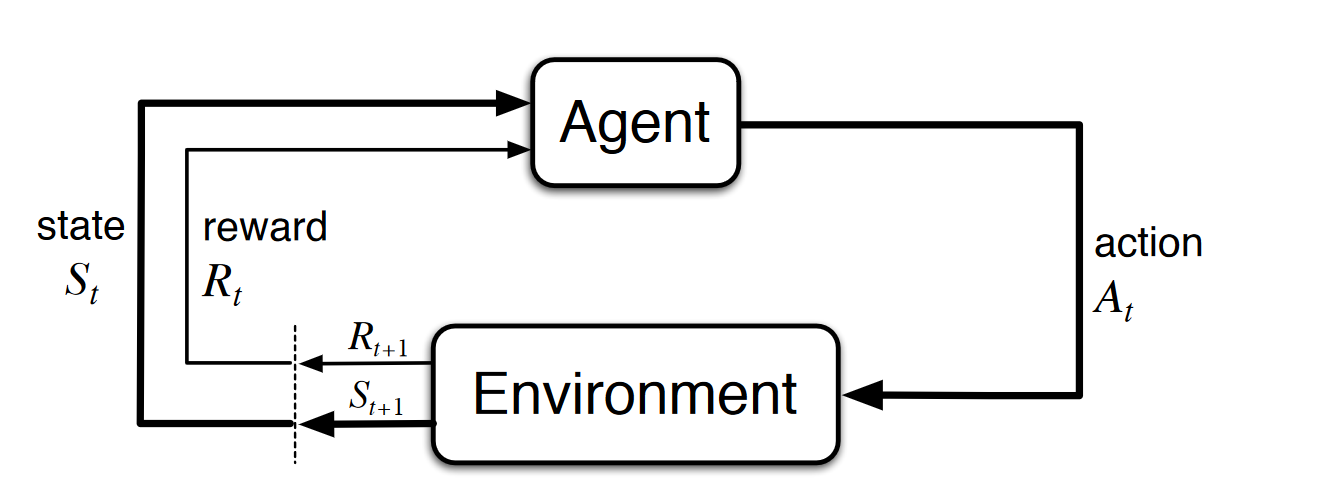
\includegraphics[height=0.2\textheight]{figures/personal_work/MDP.png}
    \caption{The agent-environement interaction\cite{sutton2018reinforcement}}
\end{figure}

In this report we will only consider the Framework of Countable MDPs and the discounted total reward criterion.
We will first start by introducing the general framework of Markov Decision Process (MPD) and the basic results on dynamic programming.

\subsubsection*{Markov Decision Process}

\begin{definition}[Markov Decision Processes \cite{szepesvari2010algorithms}]
An MPD is a tuple $\MM(\XX, \AAA, P, \gamma)$, where:
\begin{itemize}
    \item $\XX$ is a finite state space
    \item $\AAA$ a finite action space
    \item $P$ a transition probability kernel that assigns to each pair $(x,a) \in \XX \times \AAA$ a probability measure on $\XX \times \RR$
    \item $\gamma \in [0,1[$ the discount
\end{itemize}

\end{definition}

The transition probability kernel $P$ works as follow: consider a state $x$ and an action $a$, $P$ gives the probabilities to the next states and the reward received at this timestep, denoted by $P(\cdot |x,a)$. In what follows, we will write $p(x\prime|x, a) = P(\{x\} \times \RR|x,a)$ (resp. $p(x\prime, r|x,a) = P(\{x\} \times r|x,a)$) the probability to reach state $x\prime$ (resp. and receiving reward $r$) when performing action $a$ in state $x$. We also also define the random reward function $r$ so that $r(x,a)$ gives a realisation of reward obtained following $P(\cdot |x,a)$. This reward will be considered bounded almost surely. It is important to notice that the probability to reach the next depends solely on the current state and the current action. What has happened before has no influence, it is the \emph{Markov property}, that is always assumed is this Framework.

\begin{figure}[!ht]
    \centering
    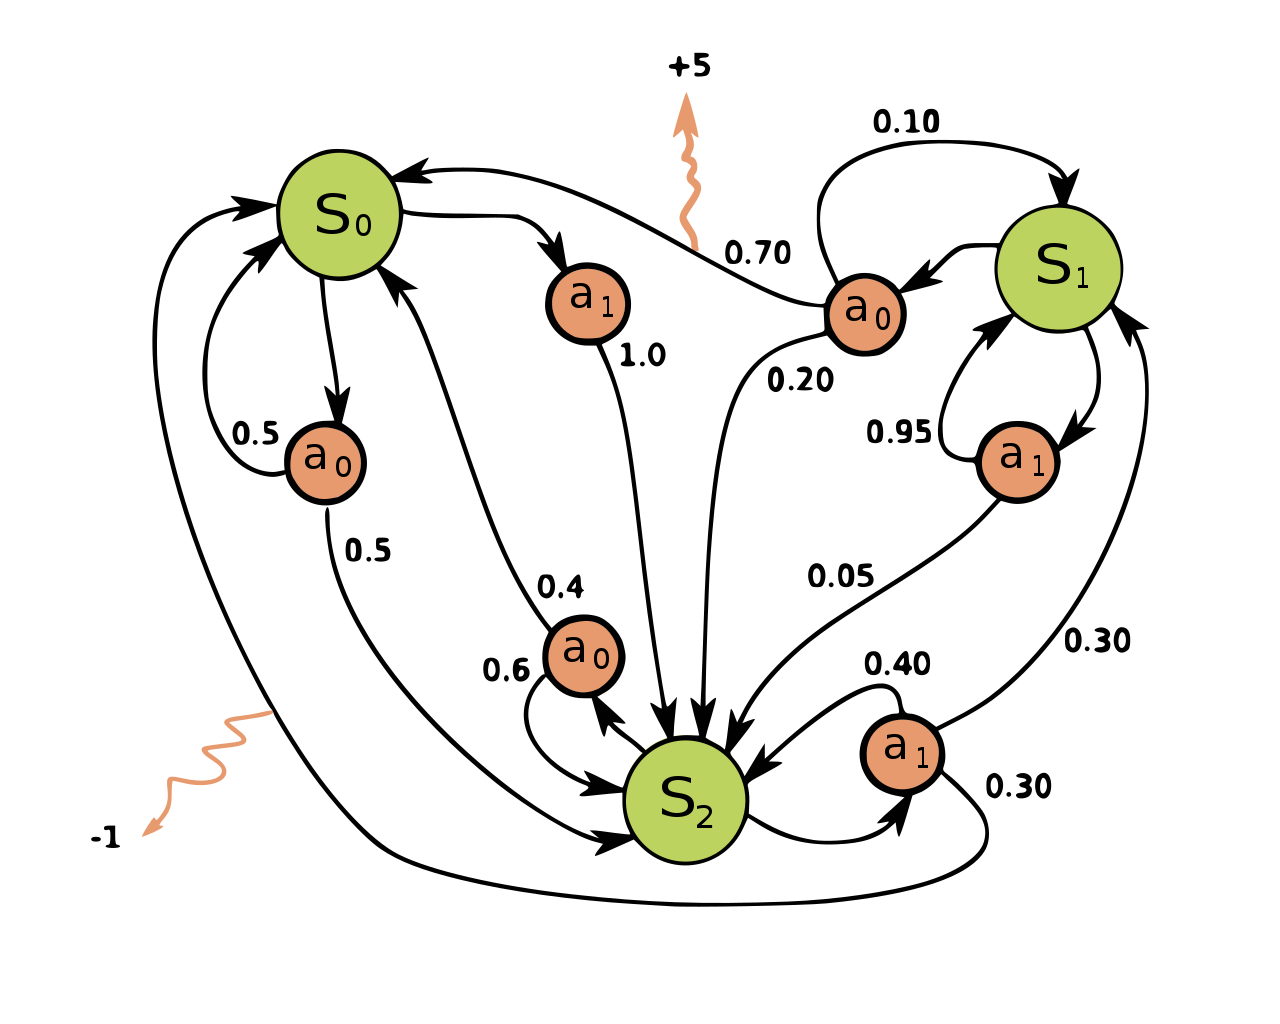
\includegraphics[height=0.3\textheight]{figures/personal_work/Markov_Decision_Process.svg.png}
    \caption{An exemple of MDP\cite{enwiki:1106395391}}
\end{figure}

The MDPs gives the formalisation of an environnent, we then need to formalize what it means for the agent to learn. We already defined a reward, that we said we wanted to maximise. However, the sequence of reward $r_0, r_1, r_2, \dots$ is random, the question is what do we maximise on this sequence. What is usually done, and what we will consider here, is to consider the sum of rewards, called the \emph{Return}:

\[ \mathcal{R} = r(x_0, a_0) + r(x_1, a_1) + \dots \]

There are two issues that arise with this definition, making it not really well defined. The first is the return being random, which is dealt with by considering the \emph{mean} of the return, giving the \emph{expected return}. The second is that, even with the expected return, we only assumed the reward to be bounded, so that return may not always be finite. This is where the discount $\gamma$ from the definition of the MDP comes to play: we consider the \emph{Discounted Expected Return} (later called simply "Return"). The goal of the agent will be to maximize this precise quantity:

\[ R = \EE{ r(x_0, a_0) + \gamma r(x_1, a_1) + \gamma^2 r(x_2, a_2) +  \dots} = \EE{\sum_{t=0}^\infty  \gamma^t r(x_t, a_t)} \]

It is now well defined and bounded: if $M$ is a bound on the reward almost surely, then :

\begin{align*}
    |R| = \left|\EE{\sum_{t=0}^\infty  \gamma^t r(x_t, a_t)}\right|& \leq \sum_{t=0} ^\infty  \gamma^t M \leq \frac{1}{1-\gamma}M
\end{align*}

The discount is important to make the sum converging, but it also has some practical implications. Because of how it is defined, the later the reward is obtained, the less worth it is. The same reward received $k$ step later is considered $\gamma^{k}$ less. Implicity, it encourages the agent to get this reward as soon as possible, to accomplish a certain task quicker. This choice is quite arbitrary but leads to a rich theory because of its computational properties and ease to manipulate.\\

We also need to emphasize on the choice of the mean. While it is a quite intuitive choice to make here and will also lead to a rich theory, it reduces greatly the information on all the possiblities, and doesn’t really take into account what happens in the extreme cases. It will require the study of the so-called "risk-sensitive" Reinforcement Learning.

\subsubsection*{Policies and value functions}

We have a formalization of the environment and a quantity we want to optimize through actions. Before dwelling in the first results of the theory, we last need to formalize the choice of actions of the agent. For that we introduce \emph{decision rules} and \emph{policies}. 

\begin{definition}
    A decisision rule $d$ is a function that maps each state to a probability distribution on the action space :
    
    \[ d: \XX \mapsto \PPPP(\AAA) \]

    It is said \emph{deterministic} if it of the form d: $\XX \mapsto \AAA$ \\
\end{definition}

\begin{definition}
    A policy is a sequence of decision rule: 

    \[ \pi = (d_0, d_1, d_2, \dots) \]

    It is said \emph{stationnary} if it uses a unique decision rule.
\end{definition}

When exploring the environement, the agent will use a policy to choose its action. It works as follows: at each time step $t$, the agent will perform an action $a$ sampled from $\pi(\cdot | x_t)$, which will lead to a reward and a next state sampled from $P(\cdot |x,a)$, then the policy gives another action, and so on.

To be able to evaluate each policies, we define the \emph{value functions}:

\begin{definition}
    The Value function $V$ is defined by:
    \[ V^\pi(x) = \EE{\sum_{t=0}^\infty  \gamma^t r(x_t, a_t) | x_0 = x}  \]
    with $x_t \sim p(\cdot | x_{t-1}, a_{t-1})$ and $a_t \sim \pi(\cdot | x_t)$
\end{definition}

This value function $V(x)$ simply represents the expected discounted reward received following policy $\pi$ and starting at state $x$. With this definition, we can now formalize the problem of RL as an optimization problem, the problem of finding an \emph{optimal policy}:

\begin{definition}[Optimal Policy]
    An optimal policy is a policy that verifies:

    \[ \sta{\pi} \in \argmax_\pi \ V^\pi(x) \quad \forall x \in \XX \]
\end{definition}

By convenience for the future, we also define the action-state value function :
\begin{definition}
    The  Q-value function (also called action-state value function) is defined by:
    \[ Q^\pi(x,a) = \EE{\sum_{t=0}^\infty  \gamma^t r(x_t, a_t) | x_0 = x, a_0 = a}  \] 
    with $x_t \sim p(\cdot | x_{t-1}, a_{t-1})$ and $a_t \sim \pi(\cdot | x_t)$
\end{definition}

\subsubsection*{A first result on the policies}

Now that the framework have been properly formalized, and before trying to compute the Value function and the optimal policies, this first result will simplify the theory

\begin{definition}[The Discounted Occupancy Measure\cite{bertsekas2012dynamic}]
    Consider the MDP $\MM(\XX, \AAA, P, \gamma)$. We define the \emph{Discounted Occupancy Measure} $p_\gamma^\pi$ by:

    \[ \forall x \in \XX, a \in \AAA, \quad p_\gamma^\pi(x,a) = (1-\gamma)\sum_{t=0}^\infty \gamma^t \PP\left[x_t = x, a_t = a\right] \]

    We then have the following rewriting of the value function:

    \[ V^\pi(x) = \frac{1}{1-\gamma} \sum_{x,a} p_\gamma^\pi(x,a)\EE{r(x,a)} \]
\end{definition}

This new writing of the value function, while seaming a bit more complicated, allows to summarize the influence of the policy in a unique term. It is used in the following results by Bertsekas:
% \begin{proof}
%     \begin{align*}
%         V^\pi(s) &= \EE{\sum_{t=0}^\infty  \gamma^t r(x_t, a_t) | x_0 = x}\\
%         &= \sum_{t=0}^\infty  \gamma^t \EE{ r(x_t, a_t) | x_0 = x}\\
%         &= \sum_{t=0}^\infty  \gamma^t \sum_{x,a} \PP\left[x_t = x, a_t = a | x_0 = x\right]\EE[r(x, a)]\\
%         &= \frac{1}{1-\gamma} \sum_{x,a} (1-\gamma) \sum_{t=0}^\infty \PP\left[x_t = x, a_t = a | x_0 = x\right]\EE[r(x, a)]\\
%         &= \frac{1}{1-\gamma} \sum_{x,a} p_\gamma^pi(x,a)\EE[r(x,a)]
%     \end{align*}
   
% \end{proof}
\begin{theorem}[Bertsekas, 2007]
    Consider a MDP $\MM(\XX, \AAA, P, \gamma)$ with the previous assumptions. For any \emph{non-stationnary policy} $\pi$, there exists a \emph{stationnary policy} $\bar{\pi}$ such that 

    \[ \forall x\in \XX, a \in \AAA, \quad p_\gamma^{\bar{\pi}}(x,a) = p_\gamma^{\pi}(x,a) \]
\end{theorem}

Combined with the rewriting of the value function, this mean that for any value function obtainend with a non-stationary policy, we can obtain the same with a stationary one. 

\begin{corollary}
    If an optimal policy exists, then the optimal policy can be choosen to be stationnary.
\end{corollary}

We can now restrain ourself to stationary policy when studying the theory further. From now on, except mentioned otherwised, all policies will be assumed to be stationary.

\subsection{Dynamic Programming}

\subsubsection*{Policy Evaluation} 

The first problem when considering a policy, is to evaluate it, \ie compute the Value function. The issue with its definition, being a mean on a infinite sum of random variables, makes significantly hard to compute directly as it is. Fortunately by using the linearity of the mean and the infinite sum, we find that the value function (and the Q-value function) verifies a recursive formula, called \emph{Bellman Equation}

\begin{align*}
V^\pi(x) &= \sum_{a \in \AAA} \pi(a|x) \left( \EE{r(x,a)} + \gamma \sum_{x^\prime  \in \XX} p(x^\prime |x,a)V^\pi(x^\prime ) \right) \\
Q^\pi(x,a) &= \EE{r(x,a)} + \gamma \sum_{x^\prime ,a^\prime  \in \XX \times \AAA} p(x^\prime |x,a)\pi(a^\prime |x^\prime )Q^\pi(x^\prime ,a^\prime )
\end{align*}

Those equations give a linear system of equation, with as many constraints as unknown ($|\XX|$ for the value function, $|\XX||\AAA|$ for the Q-value function). Which means it can be solved through matrix inversion: with $V^\pi \in \RR^{|\XX|}, r^\pi \in \RR^{|\XX|}, P\pi \in \RR^{|\XX|\times \XX},$

\begin{align*}
    V^\pi = r^\pi + \gamma P^\pi V^\pi \Longrightarrow V^\pi =  \left(I - \gamma P^\pi\right)^{-1}r^\pi
\end{align*}

This is very useful to compute the exact values in small instances, but there is another way to compute it, by iteration. For that, we will need to introduce the \emph{Bellman Operator}

\begin{definition}[Bellman Operator]
Let $V: \XX \mapsto \RR$ or $Q: \XX \times \AAA \mapsto \RR$, $\pi$ a policy. The Bellman operator $\TT^\pi$ is defined by:
\[ \forall x \in \XX, \qquad \TT^\pi V(x) = \sum_{a \in \AAA} \pi(a|x) \left( \EE{r(x,a)} + \gamma \sum_{x^\prime  \in \XX} p(x^\prime |x,a)V(x^\prime ) \right) \]
\[ \forall x,a \in \XX \times \AAA, \qquad \TT^\pi Q(x,a) = \EE{r(x,a)} + \gamma \sum_{x^\prime ,a^\prime  \in \XX \times \AAA} p(x^\prime |x,a)\pi(a^\prime |x^\prime )Q(x^\prime ,a^\prime ) \]
\end{definition}

Those operators are directly linked to the Bellman equation, which can be rewrited simpler this way :

\begin{align*}
    \TT^\pi V^\pi(x) &=  V^\pi(x)  \\
    \TT^\pi Q^\pi(x,a) &= Q^\pi(x,a) 
\end{align*}

From this we get that the value functions are fixed points of the Bellman Operators. Fixed points are essential in mathematics are allow for, under the right assumptions, for computation or proof or existence of object hard to handle. Most of it comes from the following result:

\begin{theorem}[Banach fixed point\cite{rudin1991functional}]
Let $( X , d )$ be a non-empty complete metric space with a contraction mapping $ T : X \mapsto X$. Then $T$ has admits a unique fixed-point $\sta x\in X$ and
\[ \forall x \in X, \quad T^n(x) \longrightarrow \sta x \text{ exponentially} \]
\end{theorem}

The theorem is applicable here because we get the following property:

\begin{proposition}
    The bellman operators are a $\gamma$--contractions:

    \begin{align*}
        \forall V_1, V_2 \in \RR^{|\XX|}, \quad &|| \TT^\pi V_1 - \TT^\pi V_2 ||_\infty \leq \gamma ||  V_1 - V_2 ||_\infty\\
        \forall Q_1, Q_2 \in \RR^{|\XX|\times \AAA}, \quad &|| \TT^\pi Q_1 - \TT^\pi Q_2 ||_\infty \leq \gamma ||  Q_1 - Q_2 ||_\infty
    \end{align*}
\end{proposition}

The fixed point algorithm thus gives a very simple iteration algorithm to get the value function, called \emph{Value Evaluation}: apply the Bellman Operator up to convergence with any starting values, up to a choosen point of convergence.

This algorithm will also give rise to 2 iteration algorithms to find optimal policies in a MPD.

\subsubsection*{Control} 

The second and main problem in Reinforcement Learning is to find a policy that maximizes the expected return. We to do so, the strategy will be quite similar to how we got to an algorithm for policy evaluation. First, we start by introducing the \emph{Optimal Value functions}

\begin{definition}
    The optimal value function are defined by:

\begin{align*}
\sta V(x) &= \max_{\pi} \EE{\sum_{t=0}^\infty  \gamma^t r(x_t, a_t) | x_0 = x} = V^{\sta\pi}(x)\\
\sta Q(x,a) &= \max_{\pi} \EE{\sum_{t=0}^\infty  \gamma^t r(x_t, a_t) | x_0 = x, a_0 = a} = Q^{\sta\pi} (x,a)
\end{align*}
\end{definition}

The definition of those functions can also be derived to show that they verify a recursive equation. Those one are called \emph{Bellman Optimality Equations}:
\begin{align*}
\sta V(x) & = \max_{a \in \AAA} \EE{r(x,a)} + \gamma \sum_{x^\prime  \in \XX} p(x^\prime |x,a)\sta V(x^\prime ) \\
\sta Q(x,a) & = \EE{r(x,a)} + \gamma \sum_{x^\prime  \in \XX} p(x^\prime |x,a)\max_{a^\prime  \in \AAA}\sta Q(x^\prime ,a^\prime )
\end{align*}
This equation is important not only for defining operators, but also because it leads to another theoretical results on policy. By looking at it, we notice that an optimal policy takes the action that maximizes the value function of the next state. An optimal policy can thus be chosen deterministic: this is the \emph{Bellman optimality principle}

\begin{proposition}[Bellman optimality principle\cite{bellman1966dynamic}]
    An optimal policy has the property that whatever the initial state and initial decision are, the remaining decisions must constitute an optimal policy with regard to the state resulting from the first decision
\end{proposition}

\begin{corollary}
    If an optimal policy exists, then it can be chosen to be deterministic.
\end{corollary}

Combining with the previous result on policies, although we started with very general policies, we find that the theory can be reduced to only using stationary and deterministic ones. This a specificity of the framework with the different choice that were, such as optimizing on a mean of a discounted return. We will see later that it may not be so easy in a different framework.\\

The previous results also suggests that there would only be $|\XX||\AAA|$ policies to check, but evaluating and checking them all is still quite costly. Instead, we will proceed by introducing an optimal version of the Bellman Operator, adapted to the Optimal Value Functions.

\begin{definition}[Optimal Bellman Operator]
Let $V: \XX \mapsto \RR$ or $Q: \XX \times \AAA \mapsto \RR$, $\pi$ a policy. The Bellman operator $\sta \TT$ is defined by:
\[ \forall x \in \XX, \qquad \sta\TT V(x) = \max_{a \in \AAA} \EE{r(x,a)} + \gamma \sum_{x^\prime  \in \XX} p(x^\prime |x,a)\sta V(x^\prime ) \]
\[ \forall x,a \in \XX \times \AAA, \qquad \sta \TT Q(x,a) = \EE{r(x,a)} + \gamma \sum_{x^\prime  \in \XX} p(x^\prime |x,a)\max_{a^\prime  \in \AAA}\sta Q(x^\prime ,a^\prime ) \]
\end{definition}

These operators happen to verify the same contraction properties as the previous case:

\begin{proposition}
    The optimal bellman operators are a $\gamma$--contractions:

    \begin{align*}
        \forall V_1, V_2 \in \RR^{|\XX|}, \quad &|| \TT V_1 - \TT V_2 ||_\infty \leq \gamma ||  V_1 - V_2 ||_\infty\\
        \forall Q_1, Q_2 \in \RR^{|\XX|\times \AAA}, \quad &|| \TT Q_1 - \TT Q_2 ||_\infty \leq \gamma ||  Q_1 - Q_2 ||_\infty
    \end{align*}
\end{proposition}

We can now deduce an iterative algorith, called \emph{Value iteration}: apply the Bellman Operator up to convergence with any starting values, up to a choosen point of convergence.
































% \newpage
% \subsection{unformal Distributional Approach (with random variable)[TO REMOVE]}

% \paragraph{Policy Evaluation:} 

% We here want to look at the full distribution of the return when following a certain policy $\pi$. We define the random return as follow (recall that $R$ is a stochastic reward):

% \begin{definition}[Value distribution function]
% The random value function associated with policy $\pi$ is defined as follow:
% \[ \VV^\pi(x) = \sum_{t=0}^\infty  \gamma^t R(x_t, a_t) \qquad x_0 = x \]
% \[ \QQQ^\pi(x,a) = \sum_{t=0}^\infty  \gamma^t R(x_t, a_t) \qquad x_0 = x, a_0 = a \] 
% with $x_t \sim p(\cdot | x_{t-1}, a_{t-1})$ and $a_t \sim \pi(\cdot | x_t)$
% \end{definition}

% By doing the same computation as in the expected reward case, we notice that the value distribution functions verifies an extended version of the Bellman equation:

% \begin{align}
% \VV^\pi(x) & = \sum_{a \in \AAA} \pi(a|x) \left( R(x,a) + \gamma \sum_{x^\prime  \in \XX} p(x^\prime |x,a)\VV^\pi(x^\prime ) \right) \\
% \QQQ^\pi(x,a) & = R(x,a) + \gamma \sum_{x^\prime ,a^\prime  \in \XX \times \AAA} p(x^\prime |x,a)\pi(a^\prime |x^\prime )\QQQ^\pi(x^\prime ,a^\prime )
% \end{align}

% This leads to the distributional Bellman operator:

% \begin{definition}[Distributional Bellman Operator]
% \[ \forall x \in \XX, \qquad \TT^\pi \VV(x) = \sum_{a \in \AAA} \pi(a|x) \left( R(x,a) + \gamma \sum_{x^\prime  \in \XX} p(x^\prime |x,a)\VV(x^\prime ) \right) \]
% \[ \forall x,a \in \XX \times \AAA, \qquad \TT^\pi \QQQ(x,a) = R(x,a) + \gamma \sum_{x^\prime ,a^\prime  \in \XX \times \AAA} p(x^\prime |x,a)\pi(a^\prime |x^\prime )\QQQ(x^\prime ,a^\prime ) \]
% \end{definition}

% Due to the distribution persepective, it is not possible to solve for the fixed point equation with a matrix inversion anymore. But the following result still enable theoretical computation of the exact random value distribution:

% \begin{lemma}
%     $\TT$ is a $gamma$-contraction in $d_p$
% \end{lemma}

% leads to an algorithm to find the compute the distribution

% \paragraph{Control:}

% \begin{definition}[Optimal Value distribution function]
%     \[ \sta \VV \in \{\VV^{\sta\pi} \in \argmax_\pi \EE{\VV^\pi}\} \]
%     \[ \sta \QQQ \in \{\QQQ^{\sta\pi} \in \argmax_\pi \EE{\QQQ^\pi}\} \]  
% \end{definition}

% This distribution also verify an extended version of the Optimal Bellman Equation:

% \[ \sta \VV(x) =  R(x,\sta a(x)) + \gamma \sum_{x^\prime  \in \XX} p(x^\prime |x,\sta a(x))\sta V(x^\prime ) \]
% \[ \sta \QQQ(x,a) = R(x,a) + \gamma \sum_{x^\prime  \in \XX} p(x^\prime |x,a)\sta Q(x^\prime ,\sta a(x)) \]

% and leads to the optimal bellman operator:

% \begin{definition}[Optimal Distributional Bellman Operator]
%     \[ \forall x \in \XX, \qquad \sta\TT \VV(x) = R(x,\sta a(x)) + \gamma \sum_{x^\prime  \in \XX} p(x^\prime |x,\sta a(x)) V(x^\prime ) \]
%     \[ \forall x,a \in \XX \times \AAA, \qquad \sta \TT \QQQ(x,a) = R(x,a) + \gamma \sum_{x^\prime  \in \XX} p(x^\prime |x,a) Q(x^\prime ,\sta a(x)) \]
% \end{definition}

% However, this operator is not a contraction (see Bellemare 2017). But we still have some practical theoretical results: contraction in mean. Also, convergence in sequence of optimal policy (details ?)


\subsection{Metrics}

In the next sections we will introduce the Framework for Distributional Reinforcement Learning. Before, we were only dealing with real numbers, now we will work on a space of Distribution. To do it properly, we need to introduce a few metrics.
\subsubsection*{Wasserstein Metric}

\begin{definition}[Wasserstein Metric\cite{rowland_analysis_2018}]
    Let $p \geq 1$ and $\PPPP_p(\RR)$ the space of distributions with finite $p^{\text{th}}$ moment. Let $\nu_1, \nu_2 \in \PPPP_p(\RR)$ and $\Lambda(\nu_1, \nu_2)$ the set of distribution on $\RR^2$ with marginals $\nu_1$ et $\nu_2$. The p-Wasserstein distance $d_p$ is then defined as :

    \[ d_p(\nu_1, \nu_2) = \left( \inf_{\lambda \in \Lambda(\nu_1, \nu_2)} \int_{\RR^2} |x-y|^p \ \dd\lambda(x,y) \right)^{\frac{1}{p}}\]

    Let $\eta_1, \eta_2 \in \PPPP_p(\RR)^{\XX \times \AAA}$. We also define the supremum-p-Wasserstein distance $\overline{d}_p$ by:

    \[ \overline{d}_p(\eta_1,\eta_2) = \sup_{(x,a) \in \XX \times \AAA} d_p(\eta_1^{(x,a)}, \eta_2^{(x,a)})\]
\end{definition}

This is the general definition, but it will not be practical to compute with. Instead, in our case, we have a simpler expression:

%définir la norme associé à une variable aléatoire (Bellemare)
\begin{lemma}[\cite{bellemare_distributional_2017}]
    Let $\nu_1, \nu_2 \in \PPPP_p(\RR)$ with respective cumulative distribution $F$ and $G$. Let $\UU$ be a uniform random variable on $[0,1]$. then 

    \[ d_p(\nu_1, \nu_2) = \norm{F^{-1}(\UU) - G^{-1}(\UU)}_p \]
    %\[ d_p(\nu_1, \nu_2) = \EE{\left(F^{-1}(\UU) - G^{-1}(\UU)\right)^p}^{\frac{1}{p}} \]

    which, in the case $p < \infty$ simplifies to:

    \[ d_p(\nu_1, \nu_2) = \left(\int_0^1\left|F^{-1}(u) - G^{-1}(u)\right|^p du\right)^{\frac{1}{p}} \]

\end{lemma}

$d_1$ is the one that will be used the most.

\paragraph{Cramer Distance}

\begin{definition}[\cite{rowland_analysis_2018}]
    Let $\nu_1, \nu_2 \in \PPPP(\RR)$. We define the family of metrics $\ell_p$ by :

    \[ \ell_p(\nu_1, \nu_2) = \left( \int_\RR (F_{\nu_1}(x) - F_{\nu_2}(x))^p \dd x\right)^{\frac{1}{p}} \]

    $\ell_2$ is called the Cramer distance.

    We also define the suppremum version of the $\ell_p$ norm:
    \[ \overline{\ell}_p(\eta_1,\eta_2) = \sup_{(x,a) \in \XX \times \AAA} \ell_p(\eta_1^{(x,a)}, \eta_2^{(x,a)})\]
\end{definition}

\begin{remark}
    $l_1 = d_1$
\end{remark}





\subsection{Distributional Reinforcement Learning}
%parler des résultats obtenus, pour motiver l’introduction de la notion, en plus de donner plus de possibilité sur le choix de l’optimisation.

In 2017, \cite{bellemare_distributional_2017}[Bellemare et al.] introduces the Distributional Reinforcemennt Learning framework. The idea is to compute the full distribution of the return instead of just the expected return. In his paper, they introduce the distributional Bellman operators and prove theoretical results on their properties.
\\%souligner en bleu à cause de retour à la ligne juste après une grosse expression qui prend plusieurs lignes.

The random return is the sum of the discounted random reward:

\begin{equation}
    Z(x,a) = \sum_{t = 0}^{\infty} \gamma R_t \ |\ X_0 = x, A_0 = a
\end{equation}

The idea is that the distribution of the reward would follow similar Bellman equations:

\begin{equation}\label{randvarbellman}
    Z(x,a) \deq R(x,a) + \gamma Z(X^\prime, A^\prime)
\end{equation}

with $X^\prime, A^\prime$ the random next state-action. 

\subsubsection*{Policy Evaluation}
Let’s consider a policy $\pi$. The distribution of the random return under $\pi$ will be written as follows:

\[ \eta_\pi^{(x,a)} = \text{Law}_\pi \left( \sum_{t = 0}^{\infty} \gamma R_t \ | \ X_0 = x, A_0 = a \right) \]

and we will write $\eta_\pi$ as the collection of distribution $(\eta_\pi^{(x,a)})_{(x,a) \in \XX \times \AAA}$.\\

What makes the distributional framework worth studying, is the generalization of the Bellman equation and its properties:
The random return associated to policy $\pi$ verifies the \emph{distributional Bellman equation}:
\[\eta_\pi = \TT^\pi \eta_\pi \]
where $\TT^\pi$ is the Bellman operator defined by:

\[
    \TT^\pi \eta^{(x,a)} = \int_\RR \sum_{(x^\prime,a^\prime)\in \XX \times \AAA} (f_{r,\gamma})_\#\eta^{(x^\prime,a^\prime)}\pi(a^\prime|x^\prime)p(r,x^\prime|x,a)dr
\]

with $(f_{r,\gamma})_\#\eta$ is the pushforward measure define by $f_\#\eta(A) = \eta(f^{-1}(A))$ for all Borel sets $A\subseteq R$ and $f_{r,\gamma}(x) = r + \gamma x$ for all $x \in R$.

While this operator seems more cumbersome that the non-distributional one, it just comes down to rewriting equation \ref{randvarbellman} for distributions. The proof use the exact same idea as in the non-distributional case, but in this new formalism. \\

In the tabular case, it is possible to solve this fixed point equation by matrix inversion. However, it doesn’t seem possible to do so when dealing with distribution. To solve it, we will use the following result, that is same used to solve the non-tabular non-distributional case.

Similarly as in the non-distributional case, this operator is a $\gamma$-contraction under a well chosen metric: the maximal $p$-Wasserstein metric $\overline{d}_p$ (for $p \geq 1$).

This result is very important in the sense where it gives an theoretical algorithm to compute the value distribution of a policy.

\[ \forall \eta \in \PPPP(\RR)^{\XX \times \AAA}, \quad (\TT^\pi )^n \eta \underset{n \rightarrow \infty}{\longrightarrow} \eta_\pi \]

The Wasserstein metric is important here because the same operator is not always a contraction under the total variation distance, the Kolmogorov distance or the Kullback-Liebler divergence. (ref in article de Bellemare)

Even though this algorithm seems promising, there are several issues that arise in practice, that make it difficult to implement: It is impossible to represent exactly all the space of distributions, which requires a parametrisation of the distribution and a projection step, then we most of the time don’t have access to the exact transition of the MDP, which requires a stochastic estimation of the Bellman Operator. Those issues will be tackled in the next subsections.

\subsubsection*{Control} 
Here, the goal still is to find an optimal policy. However, we will consider the full distributions of return to reach it.

We define by optimal distribution a distribution associated to an optimal policy: $\sta\eta \in \{ \eta_{\sta\pi} \ | \ \sta\pi \in \argmax_{\pi} \EEE{R \sim \eta_\pi}{R}\}$.
One of the first difference that we notice is the fact that there can be several different optimal distribution. Those optimal distribution all have the same mean, but a distribution having the optimal mean may not be an optimal distribution, because some distributions may not come from any (stationary) policy. [mettre les exemples]
 

As expected, the optimal distributions verify the optimal distributional Bellman equation: $\sta\eta = \TT\sta\eta$ with 

\[
    \TT\eta^{(x,a)} = \int_\RR \sum_{(x^\prime,a^\prime)\in \XX \times \AAA} (f_{r,\gamma})_\#\eta^{(x^\prime,\sta a(x^\prime))}p(r,x^\prime|x,a)dr
\]
where $\sta a(x^\prime) = \argmax_{a^\prime \in \AAA} \EEE{R \sim \eta^{(x^\prime, a^\prime)}}{R}$

The first interesting Control result is the fact that this operator is a contraction in average:

\begin{lemma}
    Let $\eta_1, \eta_2 \in \PPPP(\RR)^{\XX\times\AAA}$, we write $\EE{\eta}:= \EEE{Z \sim \eta}{Z}$. Then:
    \[ \norm{\EE{\TT\eta_1} - \EE{\TT\eta_2}}_\infty \leq \gamma \norm{\EE{\eta_1} - \EE{\eta_2}}_\infty \]  

    Which means that $\EE{\TT^n \eta} \underset{n \rightarrow \infty}{\longrightarrow} \sta Q$ exponentially quickly.
\end{lemma}

As before this leads to a theoretical algorithm to find the optimal value function using the whole distribution. We have another result regarding the convergence of the distribution itself:

\begin{theorem}
    Let $\XX$ and $\AAA$ be finite. Let $\eta \in \PPPP(\RR)^{\XX\times\AAA}$. Assume that there is a single policy $\sta \pi$. Then: 
    
    \[\TT^n \eta \underset{n \rightarrow \infty}{\longrightarrow} \eta_{\sta \pi} \text{ uniformly in } \overline{d}_p, \ p\geq1\]
\end{theorem}

This theorem is very important to understand how distributions behave. At first it seems really convenient, with the convergence of the distribution, but there are especially two points which are worth emphasizing. The first one is that there is no exponential convergence anymore and, in fact, the speed of the convergence is unknown. The second is the condition of unicity of optimal policy. While this condition seems reasonable, it is still possible to do without, at the cost of stationarity: if there are several optimal policy, the distribution converges uniformly to one associated to a possibly nonstationary optimal policy.

The non stationarity of the optimal policy isn’t an issue when the goal is solely to maximize the mean reward, as the greedy policy associated to its distribution will still be optimal. However, it can be more problematic if we try to find policy that takes acount of the whole distribution, such a safer or riskier policy.\\

The two previous properties are weaker that what we found in the Policy Evaluation case. To emphasize more on the differences, here are some more results that underline the pathologic cases that arise in Distributional Control:

\begin{proposition}
    The optimality operators are not always contractions.
\end{proposition}

\begin{proposition}
    The optimality operators do not always have fixed points.
\end{proposition}

The lack of contraction is the precise result that prevents us to get the same properties as in the non-distributional case or as in the distributional, especially the existence and unicity of a fixed point, and the exponential convergence.




















\subsection{Distribution Parametrization}

One of the main issue when dealing with distribution in practice, is the question of representation. It is not possible for a computer to represent the full extent of the distribution space. It is then necessary to restrain ourself on a parametrized space.

In their papers, \cite[Morimura et al.]{morimura_parametric_2012} decide to parametrize the return distribution as a Gaussian, a Laplace or a skewed Laplace distribution. Later, \cite[Bellemare et al.]{bellemare_distributional_2017} and then \cite[Dabney et al.]{dabney_distributional_2017} developed the theory for a richer class of parametric distributions, discrete ones, that are much more convenient. There two main approaches for that: the categorical approach, and the quantile regression approach.

\subsubsection*{Categorical}

This is the approach introduced by \cite[Bellemare et al.]{bellemare_distributional_2017} which led to the C51 algorithm that reached state of the art result for ALE. However, the theoretical properties of such approach were mainly developed later, by \cite[Rowland et al.]{rowland_analysis_2018}.

The idea is to use the hypothesis of bounded reward to use evenly spread diracs on that reward support, and use the diracs weight as the parameters.

\begin{figure}[!ht]
    \centering
    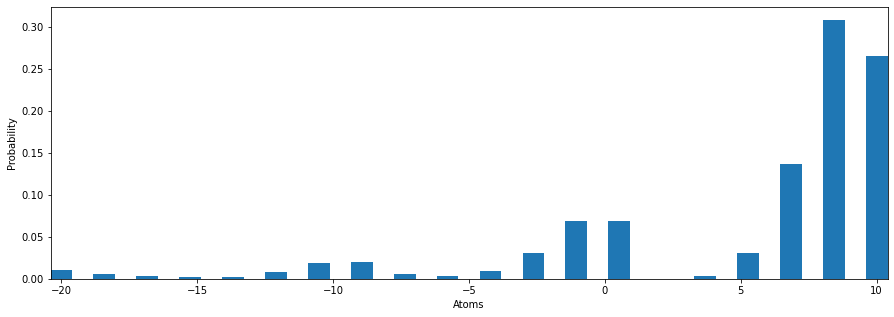
\includegraphics[height=0.2\textheight]{figures/personal_work/categoriacl.png}
    \caption{Example of a distribution projected by with the categorical approach}
\end{figure}

More formally, let’s consider $V_{\textsc{min}}, V_{\textsc{max}}$ the bounds for the reward, $N$ the number of diracs (the resolution) to use, $\Delta z = \frac{V_{\textsc{max}} - V_{\textsc{min}}}{N - 1}$ the steps between diracs. The support of the distributions will be $\{ z_i = V_{\textsc{\textsc{min}}} + i\Delta z \ |\ 0 \leq i < N \}$. The parametric family then is $\{ \sum_{i=0}^{N-1} q_i\delta_{z_i}  \ |\ \sum_{i=0}^{N-1} q_i = 1,\ 0\leq q_i \leq 1\}$.\\

%    We define the stochastic distributional Bellman operator $\hat\TT$ by :
%    \begin{align*}
%        (\hat\TT^\pi \eta_t)^{(x_t,a_t)} &= (f_{r_t,\gamma})_\#\eta_t^{%(x_{t+1}, \sta a)}\\
%        (\hat\TT^\pi \eta_t)^{(x,a)} &= \eta_t^{(x,a)} \qquad \text{if} (x,a) \neq (x_t, a_t)
%    \end{align*}
%    with $\sta a$ sampled from $\pi(\cdot|x_{t+1})$.

We define the projection operator $\Pi_C : \PPPP(\RR) \rightarrow \PPP_C$ by :

\begin{equation}
    \Pi_C(\delta_y) = 
    \begin{cases}
        \delta_{z_0} & y \leq z_0\\
        \frac{z_{i+1}-y}{z_{i+1}-z_{i}}\delta_{z_i} + \frac{y - z_i}{z_{i+1}-z_{i}}\delta_{i+1} & z_i < y < z_{i+1}\\
        \delta_{z_{N-1}} & y \geq z_{N-1}
    \end{cases}
\end{equation}
The idea behind is, for each atoms, to distribute their weight on the two closest of the projection, proportionnaly to how close they are.

Bellemare et al. introduced this projection step as an heuristic, without any theoretical motives or results related to the Wasserstein metric. It is Rowland et al. that later, found deep connection between this projection and another metric: the Cramer distance.

In fact, for the Wasserstein metric, we have the following result.
\begin{proposition}
    $\Pi_C\TT^\pi$ is not a contraction for $\overline{d}_p$ with $p > 1$.
\end{proposition}
For the case $p=1$ it is however true, but only because it is the same as the $\ell_p$ distance, for which we have much more properties:

\begin{proposition}
    For a specific subset of $\PPPP(R)$ and appropriate Hilbert space structure with $\ell_2$, $\Pi_C$ is the orthogonal projection of that subset onto $\PPP_C$
\end{proposition}
Even though the result is quite Abstract, it gives a beginning of explication on why the definition of the projection makes sense, and why it gives decent results. It also highlight the fact that this projection is closely related to the cramer distance. That distance indeed leads to better result and gives a contracting operator:

\begin{proposition}
    $\Pi_C\TT^\pi$ is a $\sqrt[p]\gamma$-contraction in $\overline{\ell}_p$.
\end{proposition}

The Banach fixed point theorem thus provides with a proof a convergence of the iterated projected Bellman operators:

\begin{equation}\label{ProjBellmanCatConv}
    \exists ! \eta_C \in \PPP_C^{\XX \times \AAA}, \ \forall \eta_0 \in \PPPP(\RR)^{\XX \times \AAA},\quad (\Pi_C\TT^\pi)^m\eta_0 \underset{m \rightarrow \infty}{\longrightarrow} \eta_C \quad \text{exponentially quickly in } \overline{\ell}_p
\end{equation}


It is important to notice that this does not have to converge to $\eta_\pi$, for the simple reason that this operator is convergent in the parametrized space $\PPP_C$, which may not contain $\eta_\pi$. The question that arises next, is how well does $\eta_C$ approximates $\eta_\pi$, question which was answered by \cite[Rowland et al.]{rowland_analysis_2018}.

\begin{lemma}
    Let $\eta_C$ defined as in (\ref{ProjBellmanCatConv}). Assume that $\eta_\pi$ is supported on $[z_0, z_{N-1}]$. Then:
    \[ \overline{\ell}_2(\eta_C, \eta_\pi) \leq \frac{1}{1-\gamma} \Delta z \]
\end{lemma}

\subsubsection*{Quantile regression}

This approach was first introduced by \cite[Dabney et al.]{dabney_distributional_2017} and led to the \textsc{QR-DQN} algorithm that outperformed C51.

The idea is to do the opposite of the categorical approach: instead of having fixed reward support with variable weight, it considers fixed weight for variable support.



More formally, let’s consider $N$ the resolution. The parametric family is $\{ \frac{1}{N} \sum_{i = 0}^{N-1} \delta_{z_i} \ | \ (z_i)\in \RR^n \}$\\

As the Wasserstein metric seems to be a metric of choice for this framework, it seems natural to try to project a distribution on the parametrized space by minimizing the Wasserstein distance between both.
In this subsection we will use the 1-Wasserstein distance. The projection operator $\Pi_{d_1} : \PPPP(\RR) \rightarrow \PPP_Q$ is thus defined by:

\begin{equation}
    \Pi_{d_1}\nu = \argmin_{\nu_Q \in \PPP_Q} d_1(\nu, \nu_Q)
\end{equation}

This is actually possible to compute, and the minimizers are exactly :

\[ \Pi_{d_1}\nu = \frac{1}{N} \sum_{i = 0}^{N-1} \delta_{z_i}, \quad F_\nu(z_i) = \frac{2i + 1}{2N} \]

where $F$ is the cumulative distribution funcition of $\nu$.

\begin{figure}[!ht]
    \centering
    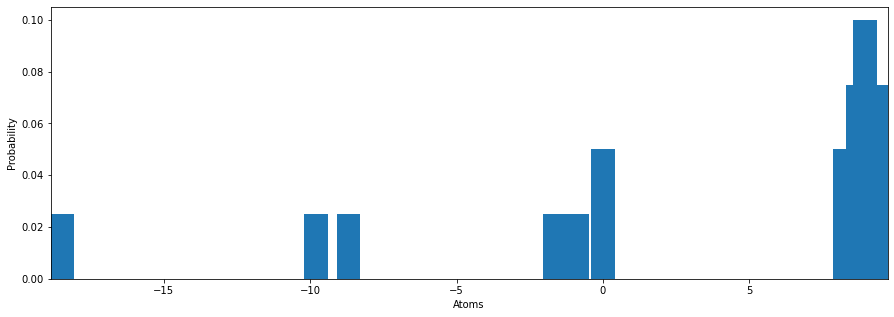
\includegraphics[height=0.2\textheight]{figures/personal_work/quantile.png}
    \caption{Example of a distribution projected with the quantile approach}
\end{figure}

This projection has the quality of being compatible with the Wasserstein metric, with which it gives a contracting operator.

\begin{proposition}
    $\Pi_{d_1}\TT^\pi$ is $\gamma$-contraction in $\overline{d}_\infty$ :

    \[ \overline{d}_\infty(\Pi_{d_1}\TT^\pi\eta_1 , \Pi_{d_1}\TT^\pi\eta_2) \leq \gamma \overline{d}_\infty(\eta_1, \eta_2)\]
\end{proposition}

This again leads to a convergence of the Bellman operator coupled with the projection step. However, no result have been found so far about a bound of distance between the true distribution of the policy and the policy it this operator converges to. The benefits of this projection is that it doesn’t require to have prior knowledge on the reward distribution, where the categorical approach requires bounds. It is thus more convenient to use.

% \subsubsection*{Diatomic AVaR}

% [Achab et Neu, motives about keeping the mean]

% \subsection{Quantile Optimization}


% Issues with greedy policy for implementation (Defourny 2008)    


% \subsubsection*{Quantile}

% [Morimura et al.]

% \subsubsection*{Superquantile}

% [results by Achab et Neu]



\section{Research Work and Results: the quantile Framework}

In this part, we are going to change the goal, and try to maximise a quantile of the distribution, instead of the mean. Indeed, sometimes we may have specific applications where the mean doesn’t matter so much, but where it is very important to have a safe policy, i.e. to have higher quantiles, even at the cost of lower mean. In the same way, it can be interesting to find more risky behavior on some environment, with higher possible reward, but at the cost of failing more often.\\

Quantile Optimization is a topic well studied in finance, in the framework of portfolios. However very few tackled this issue in the case of MDP. In their paper \cite[Morimura et al.]{morimura_parametric_2012} try to apply their first distributional approach on an Q-learning algorithm trying to optimise quantiles. Even though they obtained empirically promising results, no theoretical results have been obtained se far. A main reason for that is because quantiles are particularly hard to compute. Fearless, we will still try to tackle this topic.\\

First it is important to notice that, as the goal changed, many assumptions that were made in the original case are to be studied again in this case. The theory as to be redone from 0.

\subsection{Framework}

We are still considering MDPs of the form $\MM(\XX,\AAA, P,R, \gamma)$, but with another value to optimize. We consider $x \in \XX$ a specific state, and $\tau \in [0,1]$ the quantile of interest. Our objective is:

\[\max_\pi V_\tau(x) = q_\tau\left(\sum_{t = 0}^{\infty} \gamma R_t \ |\ X_0 = x\right) \]

Among the result that we are interested in finding back are the Bellman Optimality Principle, the sufficiency of deterministic policies and the computation of the different quantiles. Those are all results and algorithms that used some properties of the mean, mainly its linearity, which we do not have anymore.

\subsubsection*{Policy Evaluation}

The first question, just as before, is how to evaluate a policy. Let $\pi$ a policy. We want to compute:

\[ Q_\tau(x,a) = q_\tau\left(\sum_{t = 0}^{\infty} \gamma R_t \ |\ X_0 = x, A_0 = a, \pi\right) \]

When working with the mean, we would profit of its linearity to find an equation verified by this quantity, and solve this equation. Here, there is no linearity. In fact, is not even possible to compute a quantile solely knowing the quantiles for the next statest and action. We require the full distribution of the reward and the full distribution of reward and next state-action return. 

With the development of the distributional approach, we have a way to compute the full distribution of the return for a specific policy. And once the distribution is known, so is the quantile.\\

In the case where it only requires a finite number of (distributional) Bellman operator application to get the exact distribution, we get to compute the quantile exactly. This happens for instance in MDP that ends after a finite number of steps.\\

if

\[\exists k \in \NN,\ \forall \eta_0 \in \PPPP(\RR)^{\XX \times \AAA}, (\TT^\pi)^k\eta_0 = \eta_\pi \] 
then
\[ \forall \eta_0 \in \PPPP(\RR)^{\XX \times \AAA}, q_\tau\left((\TT^\pi)^k\eta_0\right) = q_\tau(\eta_\pi)\]

In the general case, even though we have the convergence of the distribution,it may not be enough for the convergence of the quantile.

\[ (\TT^\pi )^n \eta \underset{n \rightarrow \infty}{\longrightarrow} \eta_\pi \quad \nRightarrow \quad q_\tau\left((\TT^\pi )^n \eta\right) \underset{n \rightarrow \infty}{\longrightarrow} q_\tau(\eta_\pi)  \]

The result on the convergence of the operators tells us that it converges for the Wasserstein Metrics. By definintion of that metric, it means that the quantile function converges for the $L_p$ norm. However we cannot guarantee the point-wise convergence that we would need here. The closest we get is with the Riesz-Fischer theorem, that tells us that we can extract a sub-sequence converging almost everywhere. We can hope that in practice it will work well enough, which it does on the simulations.

Below are exemples of distributions evaluated for the MDP and the policies that will be introduced in the next section. They distribution parametrization was set the categorical one, with a resolution of $500$. The discount parameter was $0.9$. For the convergence, we applied the Bellman Operator $50$ times.

\begin{figure}[!ht]
    \centering
    \begin{subfigure}{0.95\textwidth}
        \centering
            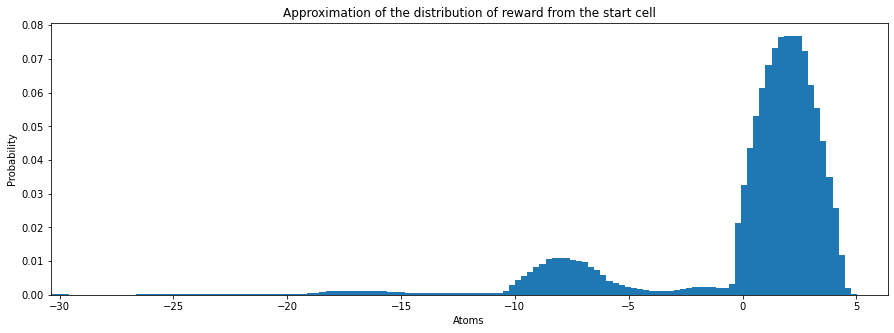
\includegraphics[width=\textwidth]{figures/personal_work/distrib_safe_policy2.png}
        \caption{Safe policy distribution}
        \label{SafeDistrib}
    \end{subfigure}
    \hfill
    \begin{subfigure}{0.95\textwidth}
        \centering
        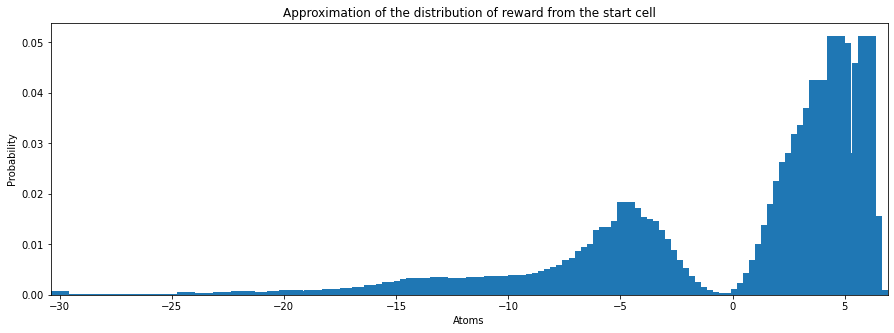
\includegraphics[width=\textwidth]{figures/personal_work/distrib_greedy_policy.png}
        \caption{Risky policy distribution}
        \label{GreedyDistrib}
    \end{subfigure}
        \caption{Examples of return distributions}
\end{figure}

\subsection{Environment of tests}

To try to understand the behavior of this new Framework we had to choose an test environment. We chose to experiment on the Cliff environment, introduced by [Sutton and Barto], which is also the one used in the article of [Morimura et al.].

\begin{figure}[!ht]
    \centering
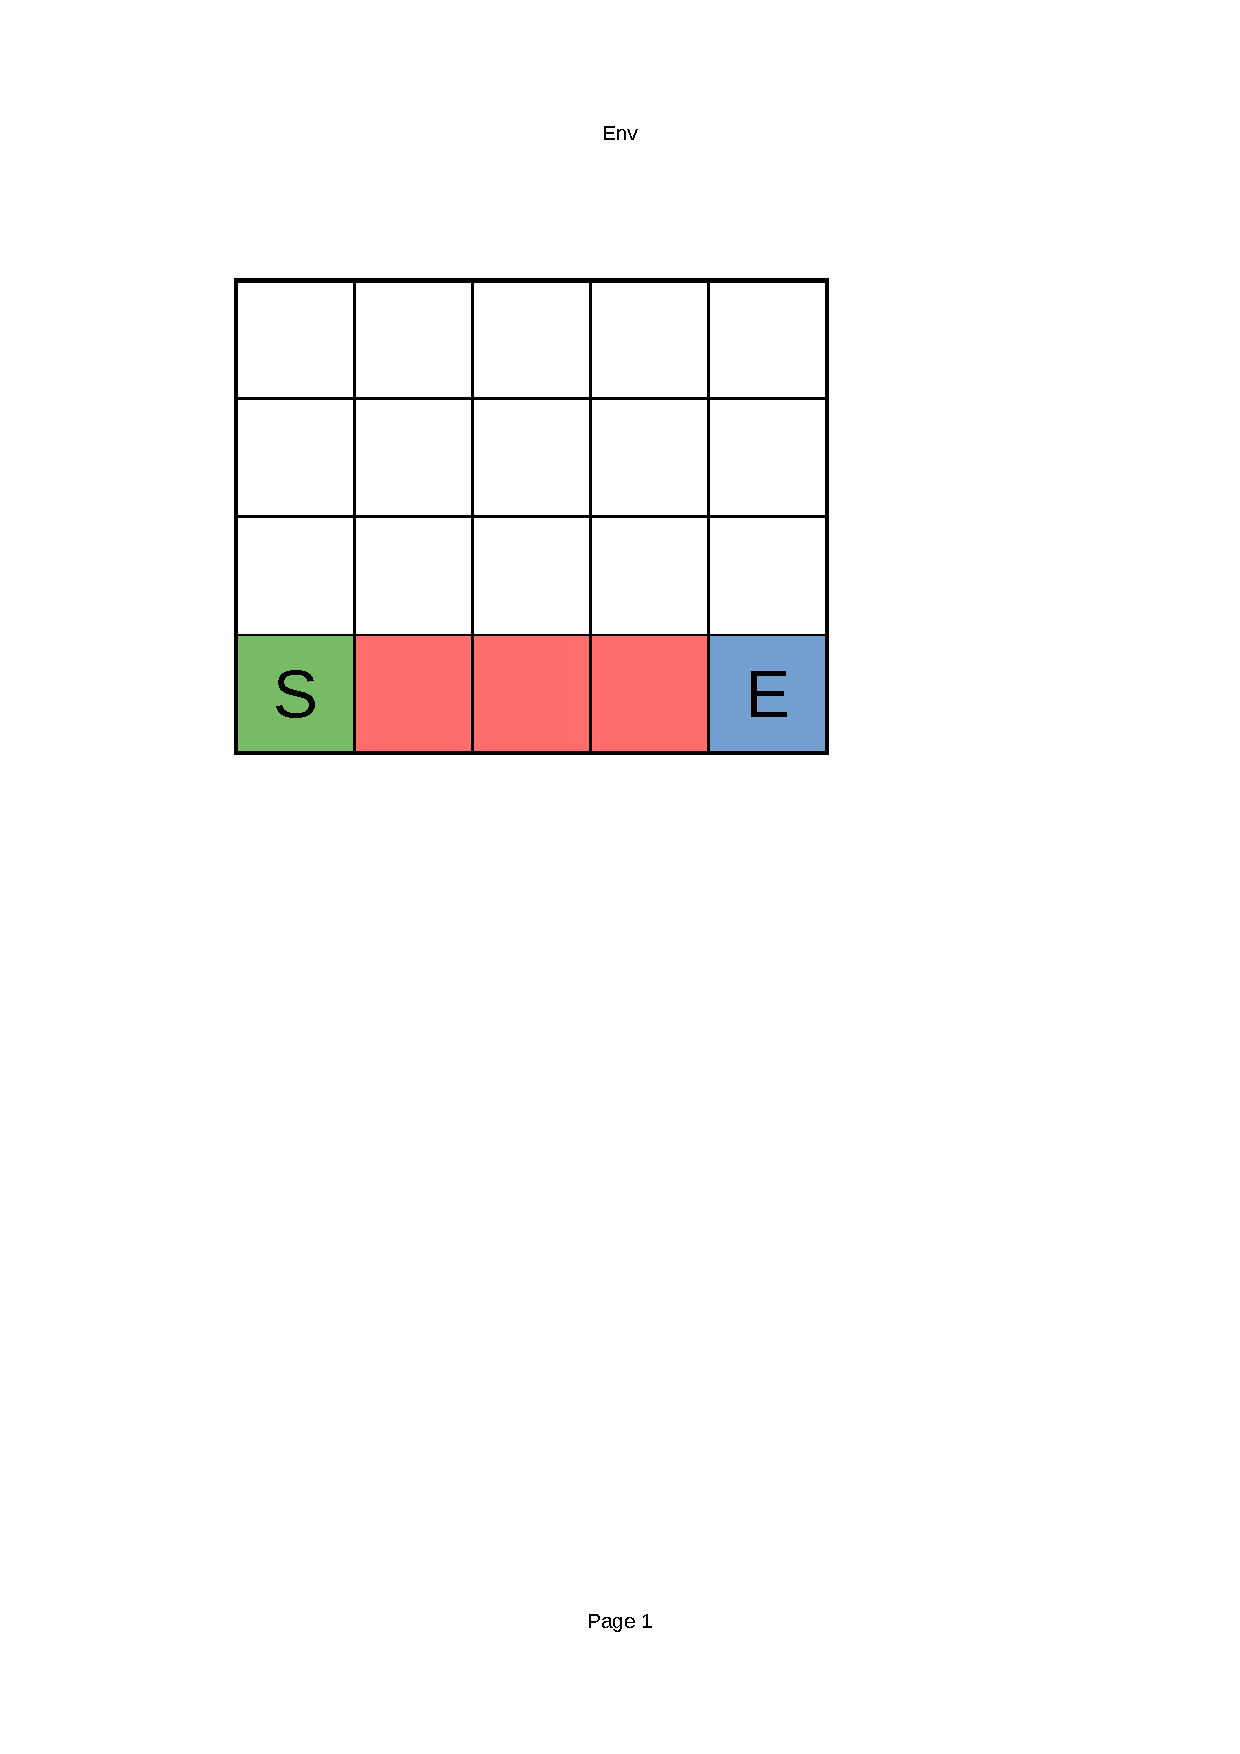
\includegraphics[page=1, trim = 40mm 160mm 70mm 45mm, clip, height=0.2\textheight]{figures/personal_work/policies.pdf}
\caption{State space of the Cliff environment}
\end{figure}

This environement is represented by a grid with a starting state (S), and a terminal state (E). There is also a pit between the two. The goal of the agent is to go from S to E without falling. The reward received when reaching E is set to $10$. The reward received when falling is set to $-10$ and when the agent does, it is teleported back to the start and has to start again. The agent can move in the $4$ directions. When it hits a wall, it doesn’t move. To add some random in it, at each step the agent has only $0.7\%$ chances to go in the chosen direction, and has $0.1\%$ chances to go any other direction.

This environment is particularly well suited for risk-sensitive RL, as it is easy to define safe and risky policy on it, making it easier to evaluate those new algorithms.

\begin{figure}[!ht]
    \centering
    \begin{subfigure}{0.45\textwidth}
        \centering
            \includegraphics[page=2, trim = 40mm 160mm 70mm 45mm, clip, height=0.2\textheight]{figures/personal_work/policies.pdf}
        \caption{Safe policy}
        \label{SafePolicy}
    \end{subfigure}
    \hfill
    \begin{subfigure}{0.45\textwidth}
        \centering
            \includegraphics[page=3, trim = 40mm 160mm 70mm 45mm, clip, height=0.2\textheight]{figures/personal_work/policies.pdf}
        \caption{Risky policy}
        \label{RiskyPolicy}
    \end{subfigure}
        \caption{Example of policies}
\end{figure}

We chose a fixed set of parameters, and tested policy iteration on it, with different optimization criterion: optimization on the mean, on the median, on the quantile 20, on the quantile 0.8. We chose the quantile projection, with a resolution of 500, we each time applied the Bellman operator 50 times (except for the quantile 0.2), the discount $\gamma$ was set to $0.99$.

The results for the mean, is the following. The algorithm converges, as expected. The optimal policy for the chosen parameters is an in-between of the safely and the safe policy. At first it acts greedily, but reaching the end, the agent find it better to just risk it and trying to get sooner, with higher risks of falling, rather than playing it safe and arriving later with a discounted reward. The importance of the discounted is highlighted when comparing with a lower discount: the agent acts more risky as taking detours decreases much more the rewards.

\begin{figure}[!ht]
    \centering
    \begin{subfigure}{0.25\textwidth}
        \centering
            \includegraphics[page=5, trim = 40mm 160mm 70mm 45mm, clip, width=0.95\textwidth]{figures/personal_work/policies.pdf}
        \caption{Optimal policy}
    \end{subfigure}
    \hfill
    \begin{subfigure}{0.70  \textwidth}
        \centering
            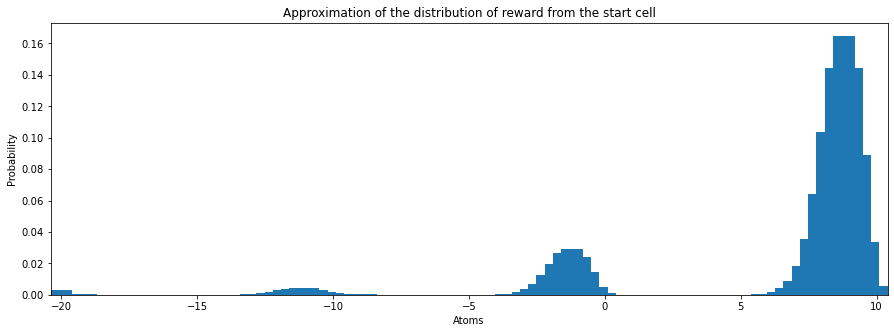
\includegraphics[ width=\textwidth]{figures/personal_work/distrib_mean_99.png}
        \caption{Optimal distribution of return}
    \end{subfigure}
        \caption{Behavior on mean optimization $\gamma = 0.99$}
\end{figure}

\begin{figure}[!ht]
    \centering
    \begin{subfigure}{0.25\textwidth}
        \centering
            \includegraphics[page=4, trim = 40mm 160mm 70mm 45mm, clip, width=0.95\textwidth]{figures/personal_work/policies.pdf}
        \caption{Optimal policy}
    \end{subfigure}
    \hfill
    \begin{subfigure}{0.70\textwidth}
        \centering
            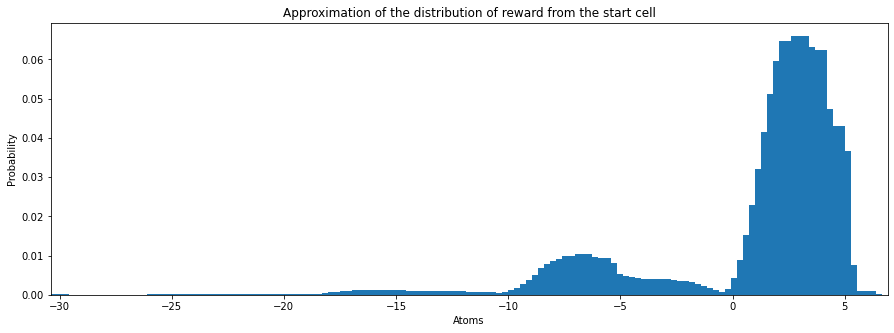
\includegraphics[ width=\textwidth]{figures/personal_work/distrib_mean_9.png}
        \caption{Optimal distribution of return}
    \end{subfigure}
        \caption{Behavior on mean optimization, $\gamma = 0.9$}
\end{figure}

The case with median is more complicated. The algorithm runs but does not converge. It ends up stuck in a loop of period 4. The following policy are what it is stuck with. On the policy we can see that at some cells, the algorithm find it better to go down. It doesn’t seem to make sens since, be it for a quantile or for the mean, it should always be better to go the right first: it gets as close to the end cell, but stay further from the edges. By analysing the value distribution function obtained, it was shown that this behavior was due to the two actions leading to the same quantile, even though going to the right was better mean-wise. In our implementation, in case of equality, the first action with maximum objective would always be chosen, which here was the down direction. In terms of theory, the quantile was equal because of the approximation necessary in the distribution parametrization, but should not be otherwise. Unfortunately, increasing the resolution would not fix the issue. Interestingly enough, this strange behavior would still result in a better median reward than the mean case.


\begin{figure}[!ht]
    \centering
    \begin{subfigure}{0.24\textwidth}
        \centering
            \includegraphics[page=8, trim = 40mm 160mm 70mm 45mm, clip, width=0.95\textwidth]{figures/personal_work/policies.pdf}
        \caption{1st output policy}
    \end{subfigure}
    \begin{subfigure}{0.24\textwidth}
        \centering
            \includegraphics[page=8, trim = 40mm 40mm 70mm 165mm, clip, width=0.95\textwidth]{figures/personal_work/policies.pdf}
        \caption{2nd output policy}
    \end{subfigure}
        \centering
    \begin{subfigure}{0.24\textwidth}
        \centering
            \includegraphics[page=9, trim = 40mm 160mm 70mm 45mm, clip, width=0.95\textwidth]{figures/personal_work/policies.pdf}
        \caption{3rd output policy}
    \end{subfigure}
    \begin{subfigure}{0.24\textwidth}
        \centering
            \includegraphics[page=9, trim = 40mm 40mm 70mm 165mm, clip, width=0.95\textwidth]{figures/personal_work/policies.pdf}
        \caption{4th output policy}
    \end{subfigure}
        \caption{Policies output by median optimisation}
\end{figure}

For the $0.8$ quantile, it converged and also led to a very greedy policy, with a higher $0.8$ quantile than in the mean case. However we still observe the issue with the agent willing to go down instead of right. 

\begin{figure}[!ht]
    \centering
    \begin{subfigure}{0.25\textwidth}
        \centering
            \includegraphics[page=7, trim = 40mm 160mm 70mm 45mm, clip, width=0.95\textwidth]{figures/personal_work/policies.pdf}
        \caption{output policy}
    \end{subfigure}
    \hfill
    \begin{subfigure}{0.70\textwidth}
        \centering
            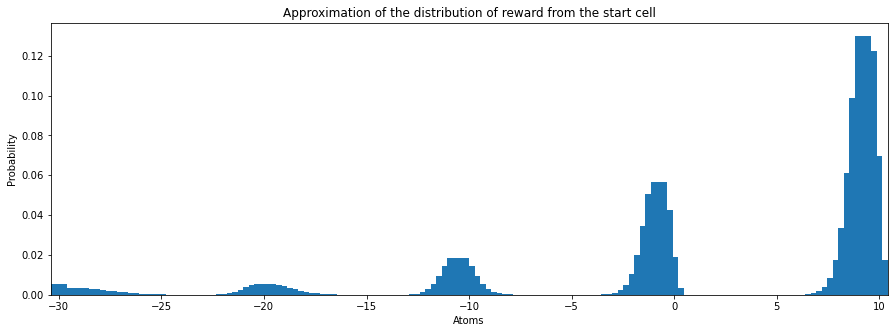
\includegraphics[width=\textwidth]{figures/personal_work/distrib_q80.png}
        \caption{Distribution of return}
    \end{subfigure}
        \caption{Behavior on 0.8 quantile optimazation}
\end{figure}

For the $0.2$ quantile, we observe a much slower convergence, needing twice as many bellman operator applications, but it did converge. We observed a policy quite similar to the one obtained with the mean. However, for this case, the algorithm output a policy that gave a lower $0.2$ quantile than the mean case.

\begin{figure}[!ht]
    \centering
    \begin{subfigure}{0.25\textwidth} 
        \centering
            \includegraphics[page=6, trim = 40mm 160mm 70mm 45mm, clip, width=0.95\textwidth]{figures/personal_work/policies.pdf}
        \caption{output policy}
    \end{subfigure}
    \hfill
    \begin{subfigure}{0.70\textwidth}
        \centering
            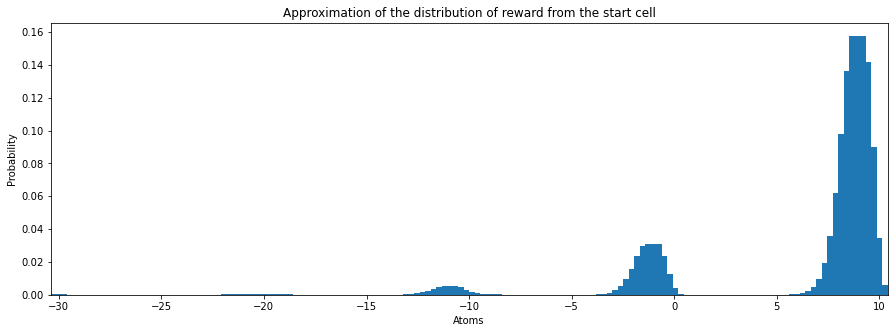
\includegraphics[width=\textwidth]{figures/personal_work/distrib_q20.png}
        \caption{Distribution of return}
    \end{subfigure}
        \caption{Behavior on 0.2 quantile optimization}
\end{figure}
In conclusion, except in a few instances, the algorithms converges and give results quite consistent with what is expected: greedy with a high quantile, safer with a low quantile. However there are cases where it does not converge. The issue seems to be the approximations in the distribution parametrization. Those approximations also lead to specific cases when quantiles are equals for differente action, which can lead to some illogical action choices. Moreover, this issue couldn’t be solved simply by increasing the resolution in the parametrization.

\subsection{Median versus Mean}

When trying to tackle to RL with quantiles, one of our question was to know how does the mean differ to the median. Often in the distribution observed in practice, both are quite close. The previous tests showed that the policy optimizing the mean could differ to the one optimizing the mean, but the median and mean obtained wasn’t significantly different. We wanted how large the difference could to know theoretically. The following example show that the difference in mean can be as high as wanted:

Here a simple example of environment where trying to maximize the median can give an arbitrary difference in mean, compared to the policy maximizing the mean. It also be adjusted to give a significant difference in the median.

\begin{center}
    \begin{tikzpicture} [node distance = 3cm, on grid, auto]
        \node (q1) [state] {$q_1$};
        \node (q2) [state, above left = of q1] {$q_2$};
        \node (q3) [state, above right = of q1] {$q_3$};

        \path [-stealth, thick]
    (q1) edge node {r = 0,M}   (q2)
    (q1) edge node {r = 1}   (q3);
    \end{tikzpicture}
\end{center}

The example consist in an initial state, and two terminal states. There are two actions, one for each terminal states. The first action leads to a reward of $0$ with probability $0.51$, and $M$ with probability $0.49$ ($M$ can be chosen as high as possible). The second action leads to a reward of $1$ with probability $1$. In this MDP, the optimal action for optimizing the median would be the second action, with mean $1$, while the first action would lead to a mean of $M/2$

This example is a great example of the dilemna that is studied when trying to minimize risks: depending on what represents the reward and the context, is it better to have low reward 100\% of the time, is it better to risk not having anything (or worse, having a penalty), but having low chances to get very high reward.

By tweaking the reward and probabilities in this example, it is possible to show that we can obtain any behavior with any quantile. Hence, in the general case, it is not possible to bound the gap between polices maximizing different quantiles and the mean.

\subsection{About dynamic programming}

Even though the approximation issues could have explained why the algorithm wouldn’t work, dynamic programming will not be able to work properly. Indeed, it worked in the general Framework because, with the mean, we had the Bellman Optimality Principle. Unfortunately, this is not the case anymore. The following MDP is a counter-example:

    \begin{center}
        \begin{tikzpicture} [node distance = 3cm, on grid, auto]
            \node (q1) [state] {$q_1$};
            \node (q2) [state, above left = of q1] {$q_2$};
            \node (q3) [state, above right = of q1] {$q_3$};
            \node (q4) [state, above left = of q3] {$q_4$};
            \node (q5) [state, above right = of q3] {$q_5$};

            \path [-stealth, thick]
        (q1) edge node {p = 0.7, r=10}   (q2)
        (q1) edge node {p = 0.3, r=0}   (q3)
        (q3) edge node {2, 3}   (q4)
        (q3) edge node {1, 4}   (q5);    
        \end{tikzpicture}
    \end{center}

On the first state, there is a single action, that have probability $0.7$ to lead to state $q_2$ with reward $10$, and probability $0.3$ to lead to state $q_3$ with no reward. Then on $q3$ There are 2 actions possible, the first one having probabilities $0.15$ and $0.85$ to get reward $2$ and $3$, and the second one, the same probabilities to get rewards $1$ and $4$. We will consider the optimisation on the quantile $0.1$. Optimizing this quantile from state $q_3$ would require to use to go to state $q_4$, with a quantile equal to $2$. However this would lead to a quantile equal to $3$ starting from state $q_1$. Doing the other action leads to a quantile equal to $4$ if starting from state $q_1$. Thus, depending on the state we start from, the actions will be different.\\

This confirms the observation that policy iteration and value iteration algorithms would not work very well in practice. There will be no guarantee that they will work on some instances of choice, and the behavior might be unpredictable. Yet, it doesn’t prevent the algorithms to output policies with better quantiles on some instances, and they could still be worse using.\\

Also, in the mean framework the Bellman Optimality Principle was quite convenient: even when wanting to optimize the return starting to a single beginning state, we would optimize it for every state simultaneously. Here, there is a choice to made, a choice on which state we want the quantile of the return optimized.


\subsection{About policies}
The first result we had on policies in the general framework, was that non-stationnary policies had the same expressive power as stationnary ones and thus, we could restrain ourself the latter. Yet, [Bellemare et al.] show that it was not the case anymore in Distributional RL, and that some distribution could only be obtained through non-stationnary policies.\\
%but what about optimal policies ?

Then, investigating the theoretical properties of the quantile framework was particularly har  because of the quantile itself. Among the few nice properties that it possess, we found this one, which has some implications with how optimal policies behave:

\begin{lemma}
    Let $n \in \NN$, let $0 \leq \lambda_1,\lambda_2,\dots,\lambda_n \leq 1$ such that $\sum_{i = 0}^{n} \lambda_i = 1$, and $\mu_1,\dots, \mu_n $ $n$ distributions. Let $q_\tau$ the quantile function for $\tau \in [0,1]$. We have:

    \[ q_\tau \left( \sum_{i=0}^{n} \lambda_i \mu_i\right) \leq \max_{1 \leq i \leq n} q_\tau ( \mu_i) \]
\end{lemma}
\begin{proof}
    Let $\mu_1,\dots, \mu_n $ probability measures. Let $0 \leq \lambda_1,\lambda_2,\dots,\lambda_n \leq 1$ such that $\sum_{i = 0}^{n} \lambda_i = 1$. Let $\tau \in [0,1]$.
    We denote $q_i = q_\tau (\mu_i)$ and $q_{max} = \max_i q_\tau (\mu_i)$.\\

    Recall that, $\forall \mu$ probability measure, 
    
    \begin{align*}
        q_\tau (\mu) &= \inf \{ x \in \RR : \tau \leq \mu ( ]-\infty, x])\}\\
                     &= \inf \{ x \in \RR :  \mu (  ]x,+\infty[) \leq 1-\tau \}
    \end{align*}

    Hence,
    \begin{align*}
        \forall i, \mu_i \left(]q_{max}, +\infty[\right) \leq \mu_i\left(]q_i, +\infty[\right) \leq 1-\tau
    \end{align*}
    since $q_{max} \leq q_i$ and by monotonicity of the measure.
    Hence,      
    \begin{align*}
        \left( \sum_{i=1}^n \lambda_i \mu_i \right) \left(]q_{max}, +\infty[\right) \leq \sum_{i=1}^n \lambda_i \mu_i \left(]q_i, +\infty[\right) \leq \sum_{i=1}^n \lambda_i (1-\tau) \leq 1-\tau
    \end{align*}
    Therefore, 
    \begin{align*}
        \left( \sum_{i=1}^n \lambda_i \mu_i \right) \left(]q_{max}, +\infty[\right) \leq 1-\tau
    \end{align*}
     which means $q_{max} \geq q_\tau \left( \sum_{i=1}^n \lambda_i \mu_i \right)$
\end{proof}

What this result mean is that, when trying to optimize a quantile, if we have the choice between different distributions and combinations of them, it is always better to only choose the distribution with the highest quantile. This is precisely the situation where are in with the MDP, on one state, we try to choose the policy that will lead to the highest quantile. This suggests that, in value iteration, we can indeed restrain ourselves to an optimal action and not having to look for all convexe combination. This also make us believe in the fact that in any MDP, we should be able to find a deterministic policy that optimizes the quantile of choice.\\

This first result is encouraging, but it is not enough on itself to show that all optimal policies can be chosen to be deterministic. We conjectured it but have only been able to prove it to some restricted MDPs:

\begin{proposition}
    Consider a finite MDP where no state can be visited twice (i.e, without any loops). Consider a state $x \in X$, and $\tau \in [0,1]$. There exist an deterministic policy $\pi^{*}_x$ that optimizes the $\tau$ quantile for state $x$ :
    \[ V_\tau^{\pi^{*}_x(x)} = \max_\pi V_\tau^\pi(x)\]
\end{proposition}
\begin{proof}[Sketch of proof]
    The idea is to write the distribution of reward starting at this state, depending on the distribution of all transition possible and with the coefficient of the policy. This lead to a convexe combination of distribution, where a distribution here would correspond to a \emph{path} in the MDP, and its coefficient would be a multiplication of several policy parameters.

    The previous result tells us that, to optimize the quantile, we can restrain ourself to only one \emph{path}. It coefficient can be set to $1$ and the others to $0$. This leads to all the policy coefficients being either $0$ or $1$, which means we have a deterministic policy.
\end{proof}

\begin{figure}[!ht]
    \centering
    \begin{tikzpicture} [node distance = 2cm, on grid, auto]
        \node (q1) [state] {$q_1$};
        \node (q2) [state, above right = of q1] {$q_2$};
        \node (q3) [state, right = of q1] {$q_3$};
        \node (q4) [state, below right = of q1] {$q_4$};
        \node (q5) [state, right = of q4] {$q_5$};
        \node (q6) [state, above right = of q5] {$q_6$};
        \node (q7) [state, right = of q5] {$q_7$};
        \node (q8) [state, right = of q2] {$q_8$};

        \path [-stealth, thick]
        (q1) edge node {} (q2)
        (q1) edge node {} (q3)
        (q1) edge node {} (q4)
        (q2) edge node {} (q8)
        (q4) edge node {} (q5)
        (q3) edge node {} (q5)
        (q5) edge node {} (q6)
        (q5) edge node {} (q7);    

    \end{tikzpicture}
    \caption{Example of an MDP on which the proposition applies}
\end{figure}

We also tested the conjecture on several simple MDPs that included loops, and everytime it seemed that the optimal policy could be chosen to be deterministic. No counter-example have been found so far. This conforts us in believing in the conjecture. However, the proof has yet to be found. The issue mainly comes from the fact that, with loops, the policies parameters appear several time multiplied to themselves, and the sum is not a convexe combination anymore, preventing us from using our only inequality on quantiles.\\

Having the most general result would be a theoretical advancement in the understanding of the framework, but may not bring much in the practical point of view. Currently, with no dynamic programming, the problem of finding the policy that maximizes a certain quantile is intractable, because of the continuum of possibilites on the policies. Looking only for a deterministic policy would help making the problem exponential in complexity (without considering the approximations necessary when dealing with distributions), which is usually too much for any real application.
%faire une section impression ? (du style, ce qui s’est passé en pratique, les difficultés…)
\section{Conclusion}
As our first contributions, we implemented a little python librairy to experiment in an easy way with Distributional Reinforcement Learning  (the code is available at https://github.com/amarthe/stageM2). This is the code used to obtain all the results mentioned in the report and, using the same parameters, they should all be reproductible. In practical point of view, this code helped illustrated how the usual tabular algorithms behaved in that new Framework, and helped us understand better the framework in general. We also contributed on the theory, by proving results and exhibiting counter-examples. We showed that Dynamic Programming was not possible on this kind of framework, when it was only assumed before, and we partly proved a conjecture stating that deterministic policy are suffiencient, which hadn’t be questioned before.

The internship was also the opportunity to try evaluate how difficult working with quantile was, and that in the future it would be better to work with difference quantities such as the expectile, which displays much better properties.\\

For the futur, there could be different ways to continue this work further. The first one would indeed be to prove or disprove the conjecture on deterministic optimal policies. Ideally it would also be to find algorithms with theoretical guarantees to evaluate and optimize the quantiles, but the theory seem currently to far behind for it to be possible. Another one would be to re-do the work of the internship but with expectiles, and improving the results further.


\newpage

\bibliography{citation} 
\bibliographystyle{ieeetr}

\end{document}
